\documentclass{article}
\usepackage[a4paper, margin=3cm]{geometry}
\usepackage{graphicx}
\graphicspath{ {./pics/} }

\begin{document}

\section{Playtesting}
The first game concept I came up with was a turn-based three-dimensional boardgame. I built a physical prototype from paper, chess pieces and other pieces. To simulate a three dimensional space, I drew grids on three papers witch I put next to one another. 

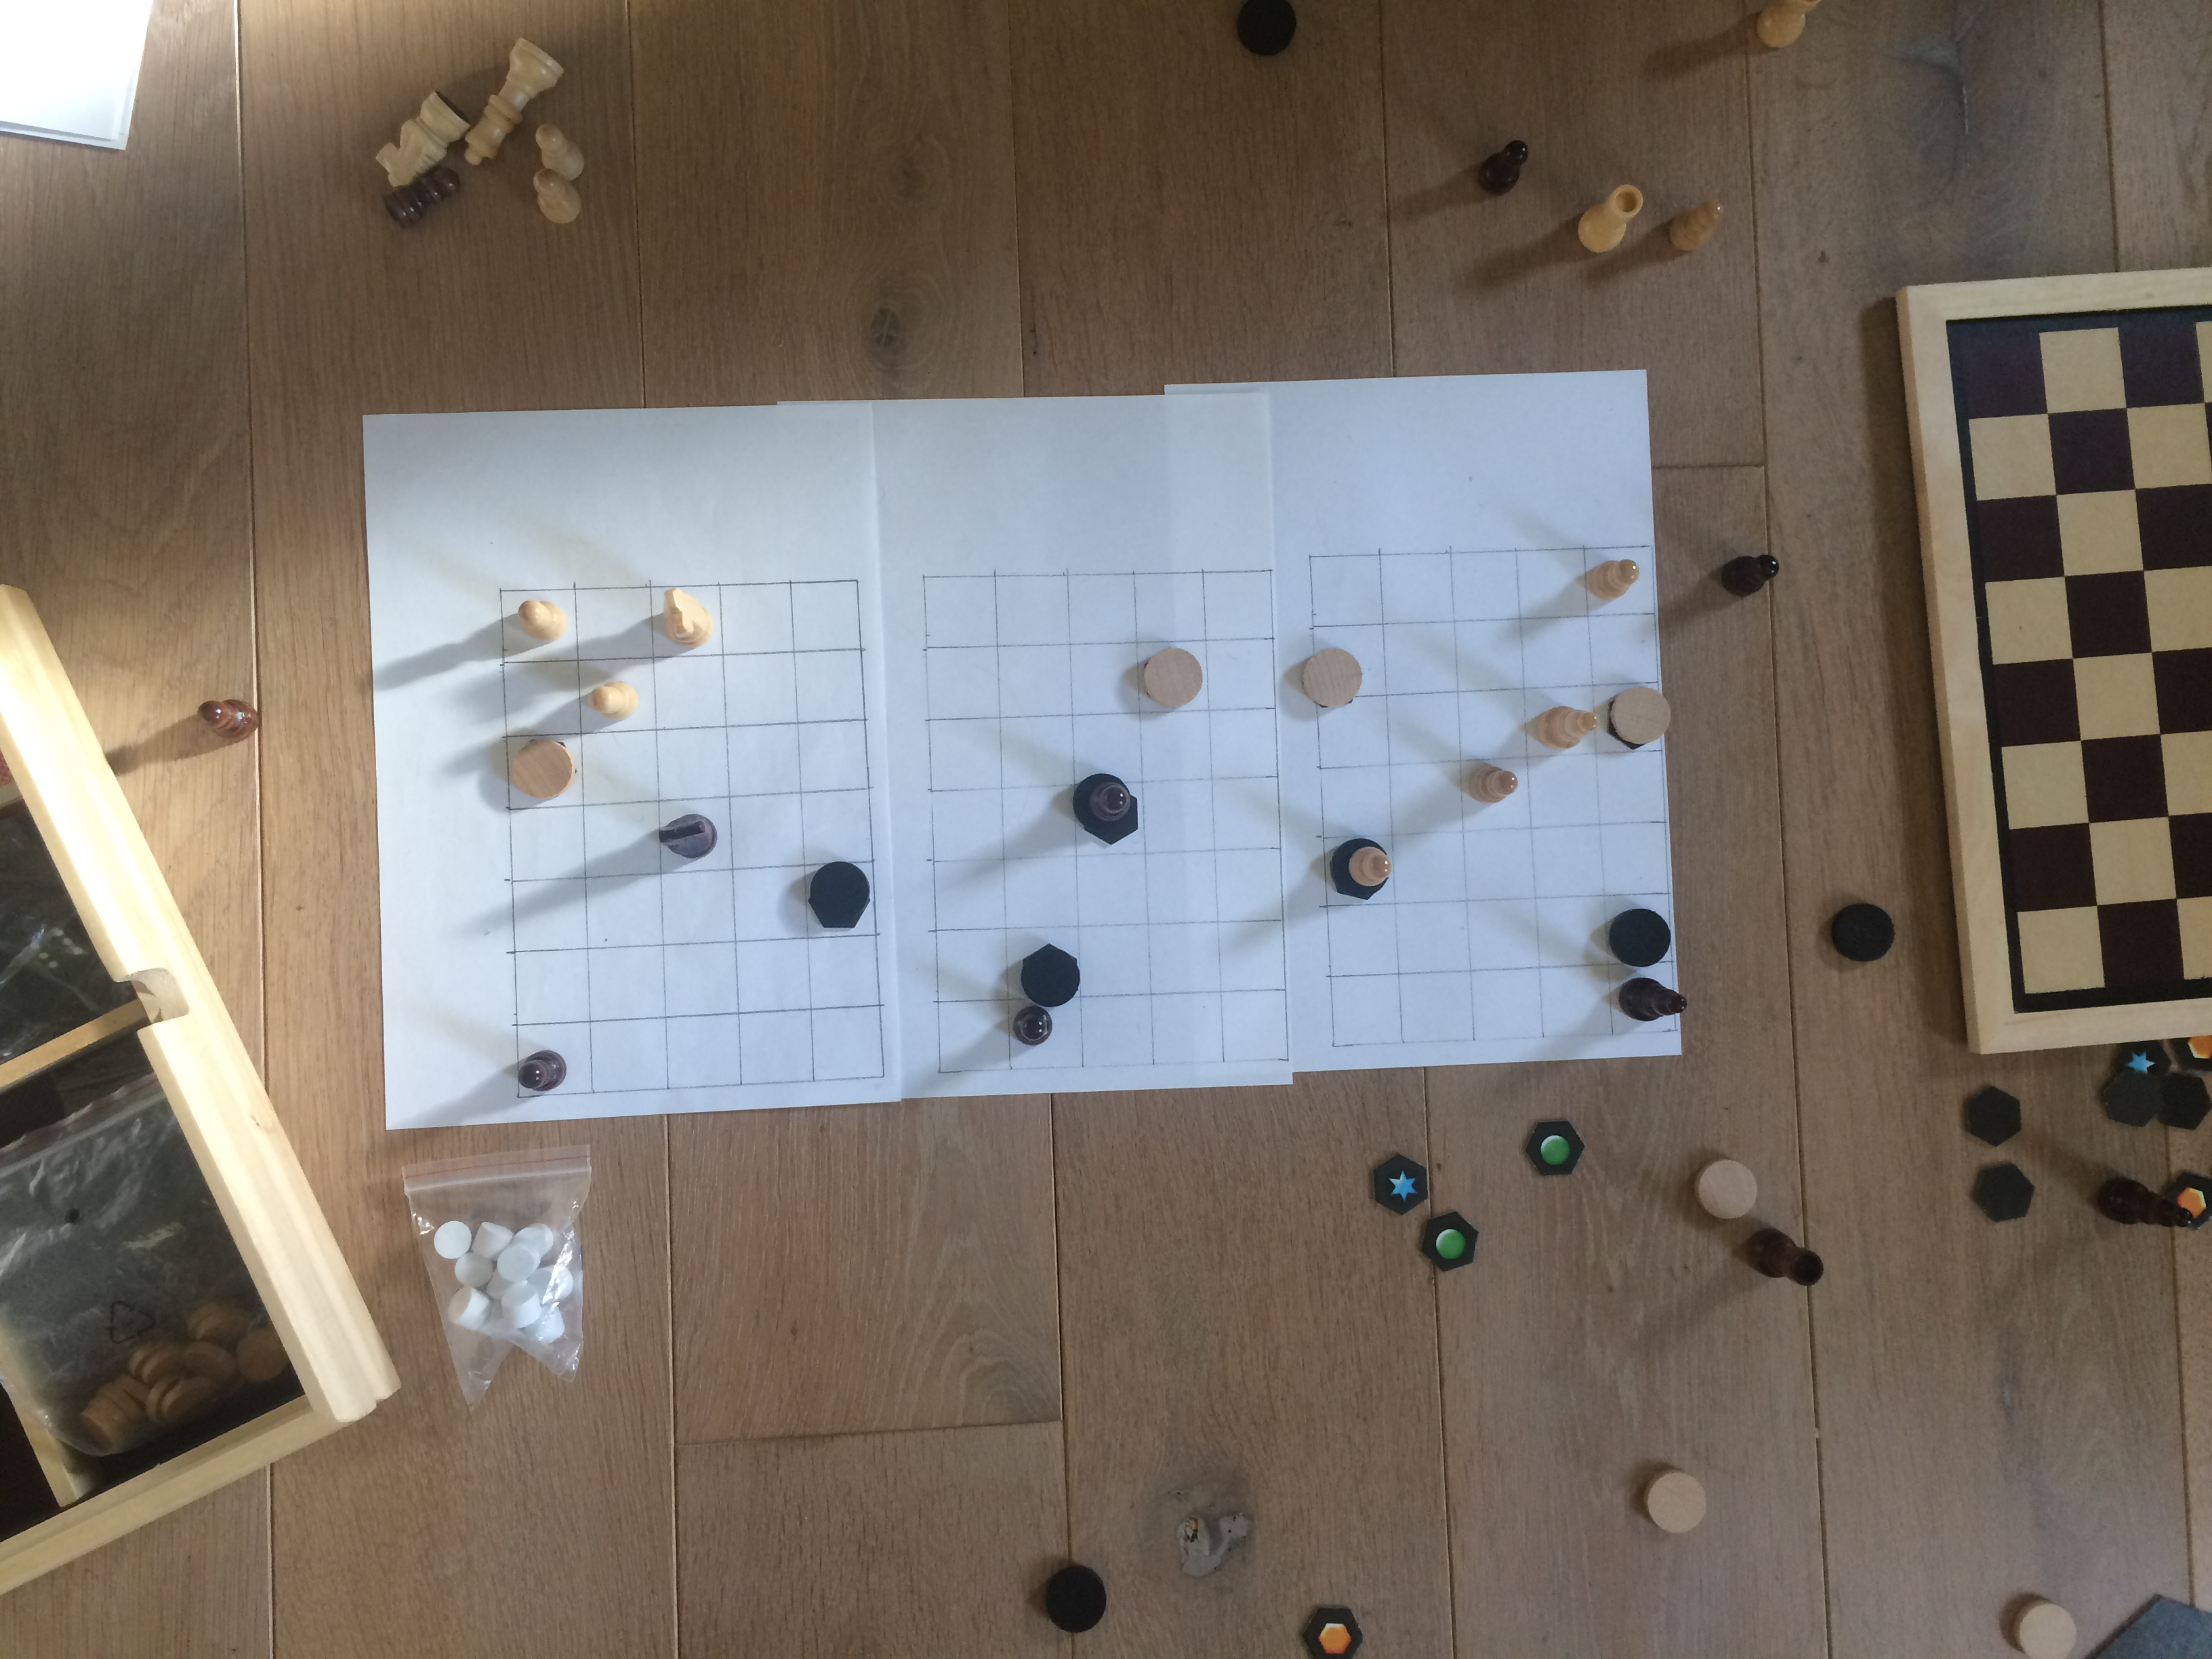
\includegraphics[width=10cm]{prototype}

Initialy, I was moving the pieces around and tried to come up with rules, which didn't quite work out, so I asked my brother to play with me (that was on Feburary 26). With some initial difficulties (he didn't quite know what I was expecting him to do), we finally came up with a set of rules. Two days later I asked another family member for help so that I can try out different variations of the game, including a hexagon based board and different starting positions. Playing the game with a different person was a completely different experience, and a lot of flaws were discovered in the rules. The biggest issue was that my playtester didn't quite understand the goal. Due to this experience, and my insistance on using GoDot as a game engine, which, as I learned, might not be the best choice for 3D games, I chose to opt for a different idea: a seagul simulator.

\bigskip
The next concept was about stealing food from other people and completing quests. I did draw a map on paper and made some seagulls and humans from cardboard, tested it out myself, and two days later, I conducted another playtesting session with my brother. Stealing food became boring very soon, however he was very motivated to complete quests. 

Once I was confident that the game idea had potential, I started to build a quick digital prototype. I quickly realized however that the art style I was using, which was pixel art, was causing me a lot of issues: it was very difficult to find good assets, especially because I couldn't draw them myself, and the assets had different resolution, meaning that they didn't match at all. Frustrated and not willing to get any more headaches from aesthetical issues, I descided to change the game concept again.

\bigskip
I finally found a complete asset pack that I liked, and I descided to create a multiplayer platformer. I didn't do any physical prototyping, but created a digital prototype to create levels for assignment 1, which helped me a lot to test the gameplay for myself. 

Then, I started to implement the authentication system first, and the invitation functionallity and lobby afterwards. Once this was done, I started to implement the actual game. 
Looking back at how I approached the project, it would have been much better if I had initially focused on the actual game itself, and not implementing user screens first. This approach would have allowed me to start with the playtesting process much earlier. Moreover, it would have forced me to think about encapsulation and decoupling right from the start. 

\bigskip
On April 18, I run the first digital playtesting session, in which I wanted to find out if the game was overall playable. Authentication, inviting players, starting the game from a lobby and playing two levels, as well as switching to the next level, did already work at this stage. It should be noted that the bridge in level 1 did still work as was described in the project plan. My brother and his girlfriend happily volunteered to play the game on two separate computers. Just like in the remaining session, I started off by telling them how playtesting is going to help me, that it's an unfinished prototype and that all their mistakes are going to help me. I also asked them to think out loud.
I continued by asking question about their gaming habits: my brother regularly plays FPS, his girlfriend nothing. 

Opon loggin in, they were confused by the font which is all capital letters. I later changed the authentication system to treat everything as lower case letters, which solved this issue and has the benefit that players with usernames that only differ in case cannot be accidentally confused anymore, an issue that occurs with almost every system that supports usernames.

To my surprise, when trying to send out an invitation and starting the game through the lobby (which still existed at this point), they managed to break the system in ways I never imagined to be possible. In the end, I had to intervene and start the game for them.

They mentioned that it would be great to have a screen that shows the available controls, however I chose to not implement this suggestion yet.
They were also trolling each other in different ways, a behaviour that would have been great to encourge, however I didn't encounter this in the following playtesting sessions.

In the second level, they found a way to use the spring board in a way that wasn't intended. Due to the way the code worked at that time, they could simply stay on the board and their character would always jump a bit higher once he landed on the board. A variable was modified later on so that a player who jumps onto a spring board cannot jump any higher than the height that he had before jumping onto the board.

Once the playtesting session was over, I asked them question about the game. They had the assumption that they'd both needed to enter the exit at the same time, which was changed later on based on their feedback. As the second level was a bit hard, they needed around seven attempt to reach the exit. When asked, they confirmed that they were positively surprised by the difficuly, which motivated them to finish the level.

\bigskip
The next day, I was doing a less formal, remote playtest. This time I wanted to find out if it was possible to play the game with someone who's not on the same network as I am. I did setup port forwarding on my router at home so that the game servers could be reached from outside. The playtester shared her screen so that I could see what she was doing. 

Upon reaching level 2, she didn't understand how the spring board would work, so I eventually had to explain it. The goal was to make the board as intuitive to use as possible, so I added another spring board at the beginning of the 2nd level. 

Moreover, as her screen was quadratic, she couldn't see certain elements that I could see, an issue that I haven't thought about before.

\bigskip
I then organised another two playtesting sessions, both on the 23th. It would have been better to have them on two separate dates, but this wasn't possible due to organizational issues.

\bigskip
The next session was a remote session with two of my friends that don't play video games.

Surprisingly, they didn't understand that the buttons were colour coded. In order to make this concept more intuitive,  I put two buttons with different colours next to one another right in the beginning of level 1 and changed the bridge's code to stay visible once both buttons were pressed.

The also had issue with spring boards because were too tiny for them and they didn't quite understand the way they work, so I increased their size.
Moreover, when they realized that they had to try the second level again because they fell off, their motivation was immediately gone, which is why the second level is now a bit easier to satisfy non-gamers alike.

Another issue that is worth mentioning is that on one playtester's screen, the other player's character was not at the position where it was supposed to be but it rather moved all over the place. I attributed this issue to a bad internet connection

\bigskip
When doing the next playtesting session, the aforementioned issue occured again, but impacted the gameplay so badly that it was impossible to properly test the game. I then asked each playertester to connect with a client that was running on my computer. I found out that my client run perfectly well, which I attributed to the server running on the same machine. Only one client had this issue, so I had to test the game with one playtester only. I decided to not fix this issue and focus on other aspects in the development because it would have been a very difficult endeavor to spot this issue and check if it's working because I don't have the capacities to test on another network and to get many more people who would be willing to test the game.

It should be noted that, due to didactical issue in the session earlier that day, this version had coins, which I hope could guide the player and teach them how the spring board is to be used, which was confirmed by how the player played.

\bigskip
I also tried to playtest the game with people that I don't know by putting on a post in the playtesting channel in the Module's Teams Group, however I didn't get any replies, which is why this game was only tested with people I know.


\section{Changes from project plan}
Firstly, on the playerList screen, I only included a list that shows players which are currently logged in and not playing a game. It took significantly more time than I expected to set up the aforementioned list properly, and because a friend system wouldn't be necessary for the game to work, I descided to omit this feature. 

\bigskip
Moreover, I also removed the entire lobby screen. At some point in the development, I realised that the server side code was very messy and tightly coupled, which constantly caused bugs with the lobby and player list features. Then I decided to decouple and refactor the entire server code, which took quite a while. Because the lobby wasn't finished and not necessary for the game to work properly (as the friend system, it could be added in a theoretical future version of the game), I descided that it would be best to remove it entirely and to focus on the player list feature first (which still has some bugs, unfortunately) and to focus on play testing, which was pretty time consuming as well.

\bigskip
On the playerList screen, there is now a text which shows the name of the currently logged in user, which is helpful for debugging purposes and for players alike.

\bigskip
Regarding the game itself, I did modify the levels quite strongly based on how players interacted with the levels. Moveable boxes, like the ones planned in level 2 were also removed as I chose to focus on other issues. As mentioned in the playtesting section, I added the option that platforms can appear and stay visible if two players simultaneously step onto the buttons. 

\section{Design Patterns}
The Client Project uses Godot's build-in architectural design pattern, which, compared to a classical ECS, uses Nodes instead of entities with components, favours inheritance over composition, while still allowing the later to be used on a higher level, and, similar to systems in ECS, uses what the Godot developers call servers and lets Nodes have their own logic in the form of scripts. 

This architectural pattern was mainly chosen because Godot is build around this pattern, thus being well integrated with Godot's design philosophy, making it very userfriendly and leightweight, while still providing good performance. Moreover, as there is no destinction between scenes and prefabs - everything is a node in godot - it become easier to combine and compose nodes which increases the reuse of parts of the game. Considering the complexity of the game there should not be any performance issues compared to a traditional ECS approach, however if optimization was required in the future, it would easily be possible to do so, for instance  by only processing visible objects or by directly interfacing with Godot's low level servers for critical game code. 

This pattern can be seen almost everywhere in the Client project. For instance, the scenes in the Levels folder make heavy use of this pattern. They all inherit from the superclass Level, which provides funcionality common to all levels. Composition can still be found in the individual level nodes, which hold different nodes that make up the level, such as platforms or pressure plates.

\bigskip
In order to decrease coupling between objects, I used Godot's build in signaling system, which acts as an observer pattern. It is everywhere for communication between nodes where a Composition or Aggregation cannot be assumed, or when making calls to a Singleton. 

This can be found in the Services.gd Singletons of both the Services and the Client project. When receiving a remote procedure call, they simply emit a signal. Before refactoring the entrie Services project, thich was done with Singletons and simple function calls, which made it very difficult to get invitations to work properly or to extend anything. 

Moreover, every pressure plate that inherits from PressurePlat.gd emits a custom signal when a player enters or exits it's area. This signal is then connected with an object that includes Platform.gd, such as Bridge.tscn, to trigger the Platform to be shown or hidden based on it's properties. As a side note, Platform.gd also makes use of the Command pattern by using a FuncRef to call the perform the correct action, hide or show, based on the objects properties.


\bigskip
I made use of the Singleton pattern. Initially, I used way too many Singletons, which resulted in high coupling, especially in the Services project. Stritcly speaking, an Autoload in Godot, which I'm using as a Singleton, can be instanciated multiple times and is therefore, strictly speaking, not a Singleton.

Singletons are used for every script that has a NetworkMultiplayerENet: Gateway.gd, Authentication.gd, Services.gd and TokenTransfer.gd. Using Singletons in this context makes sense as the rpc's can only call functions on a remote machine that have the same Node path, and Singletons guarantee this. Moreover, the networking functionality is expected to stay available during the entire game and needs to be accessible by every other Node. It might make sense to only call functions on the Networking Singletons only with signals, however as these nodes are assumed to always be available they're called directly.

Singletons are also used to hold global information, such as the game\_id or the players username in Global.gd in the client project, or to provide an interface to another API, such as Database.gd in Authenticate which provides methods to manipulate the underlaying database (Please note that in this case there in no database connected, but all data is stored in json plaintext on the same machine, however as the interface stays the same, one could easily connect the project with a database)

\section{Networking}
Networking is done through godot's high level multiplayer API, which is mainly using remote procedure calls. I decided to implement a client-server model, and not a peer-to-peer game, mainly because that is what interested me most and because this architecture allowed me to play the game with people that are not on the same network.

As mentioned previously, all networking related functionality can be found in Authenticate.gd, Gateway.gd, TokenTransfer.gd and Services.gd.

Each player is sending its position every frame to the game server (Services). Services is then sending the game state, consisting of every player's position, to all client at 20 fps (due to performance considerations). When a client is receiving a world state, it is rendering the game 100ms in the past. Packets that transport the world state may get lost in transit because an unreliable protocol was used to reduce the extra time that a reliable protocol like TCP would take for handshakes. As these packets may get lost, and because packet might not and will not arrive at the same frame rate as the client is rendering at, it is necessary to interpolate and extrapolate between world states, which is the reason why clients are rendering 100ms in the past.

The client will also notify the server using a reliable protocol when it triggers an action, for instance when it enters or leaves the exit area or when it leaves the game.

The is no server-side map implemented. As a result, the game server acts more like a proxy for two peers that are on a separate network, which is a very interesting concept that I haven't seen many games implementing. However, this also means that I'm facing most security issues that peer-to-peer games face, most notably that there is no central authority which checks if the players are cheating. I think that the issue mentioned in the playtesting section (the other character is changing its position to any place on the screen at a very fast rate) is due to the absence of a server-side map and an authority which checks for the validity of player states. 

I only realized the occasional impact on the gameplay and the security issues that were associated with this design descision fairly late in the development process during a playtesting session. Considering that it would have been a major endeavor to implement a server-side map at this late stage, I descided to accept these flaws and focus on improving gameplay.

Knowing what I know now, I would have implemented a server-side map and security checks right from the beginning, especially because that is the major advantage of a central server. Additionally, if I were to do such a project again, I would do more reading on the concepts and I would follow less tutorials. Tutorials are great to get started, but I think that it would be better to create two or three more prototypes to explore concepts such as server-side maps more in depth.


\section{Security Considerations}
The major security aspect which I considered is authentication. To increase security, I opted to create a different projects for the server which checks credentials agains a database (Authentication), a Gateway which forwards authentication requests from Client to Authentication and back (Gateway), and a server on which multiple instances of the game run and services such as a feature to invite player are managed (Services).

When the client wants to login or create an account, he's sending the username and an encrypted password to the gateway server, which in turn connects to the Authentication server. The gateway is adding another layer of security as no client from the outside can directly connect to the authentication server. The authentication server is then verifying the credentials against a database (Which is just a simple json file for the time being, but could be replaced with an actual database in the future). If the credentials are correct, it generates and timestamps an authentication token and sends it via TokenTransfer.gd to the Services server and through the gateway to the client. The client then authenticates with Services through Services.gd by sending the authentication token that it received from the gateway. If the tokens match and the client authenticates within 30 seconds after the token was generated, the player is authenticated. 

All communication, except between Client and Services, is encrypted using the Datagram Transport Layer Security (DTLS). 

In order to implement this feature, I created a new project CertGen which generates and saves a self signed x509 certificate and corresponding RSA key to its user:// directory. These files where then renamed and for every script that acts as a server, both the certificate and key were moved into a folder of the corresponding project and were included by the server script, and the corresponding certificate was copied into the Resource folder of the corresponding client in a different project. For instance, for gateway.gd, a client script from Client, and gateway.gd from Gateway, which acts as a server, the files cert\_gateway.crt and key\_gateway.key were move into Gateway->res://Resources/Certificates, and key\_gateway.crt into Client->res://Resources/Certificates.When a network peer is created, the setting dtls\_enabled is set to true and the key and certificates are connected with the corresponding network peer..

The reason for not encrypting communication between Client and Services is that encryptinge game data would take too much time. Moreover, protection agains hacking is done by the server, and would be even more improved if there was a server-side map, as already mentioned. There is still the chance of a man-in-the-middle attack when the token is transfered. This risk still exists because I couldn't find a way to toggle between encryption and plain text in Godot's Multiplayer API.Encrypting everything would not have been an issue because that would result the game in being impressively slow. However, the attacker would only be able to get a token, which only last 30 seconds, and cannot deduct the password from it. 

As mentioned previously, there is very litte validation of player states because there is no server-side map implemented. As said previously, a server-side map would have taken care of most error checking by simulating the player movement with its physics engine.

\section{Notes}
Before playing the game, authentication.x86\_64 should be executed on the server first, then gateway.x86\_64 and services.x86\_64. Once this is done, the clients can be started. The client connects to servers at 127.0.0.1 by default. To change this behaviour, modify user://config.json (Please note that the file is created the first time your run the client, but can also be created it manually).

\end{document}
